\begin{frame}{The binomial distribution: when it fits}
\begin{columns}[T,onlytextwidth]
\begin{column}{0.48\textwidth}
\onslide<1->{
\centering
\textbf{Larry Bird: pairs of free throws} \\
{\footnotesize 338 pairs, 1980--82} \\[4pt]
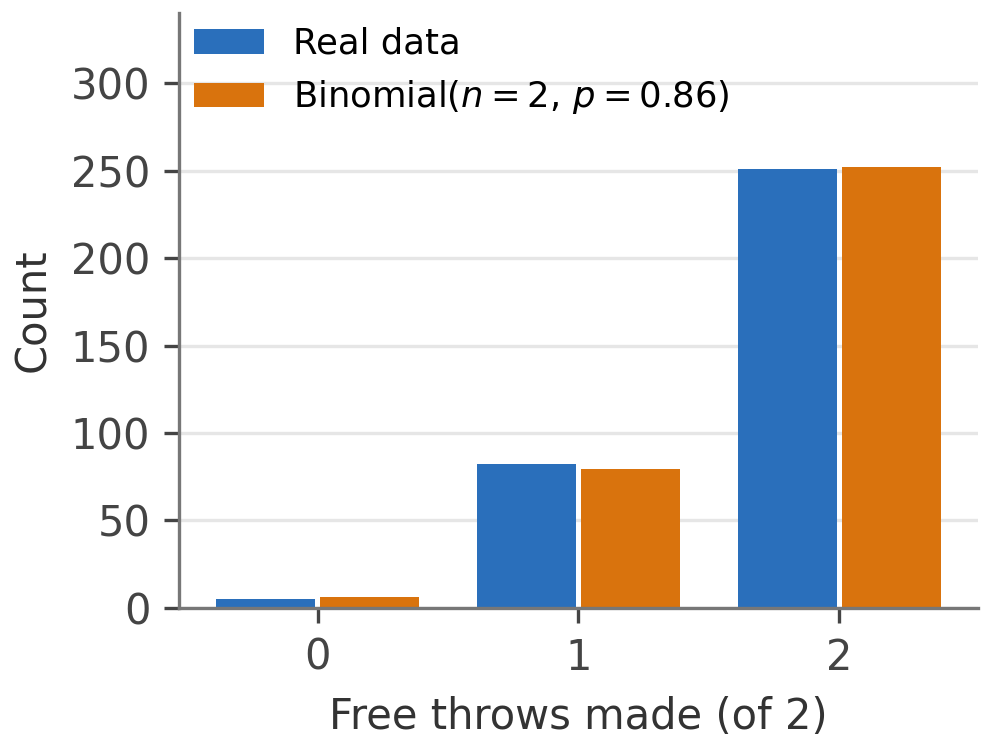
\includegraphics[width=\textwidth]{images/binomial_fit/bird}
}
\end{column}
\begin{column}{0.48\textwidth}
\onslide<2->{
\centering
\textbf{Ichiro: games with 4 at-bats} \\
{\footnotesize 931 games, 2001--12} \\[4pt]
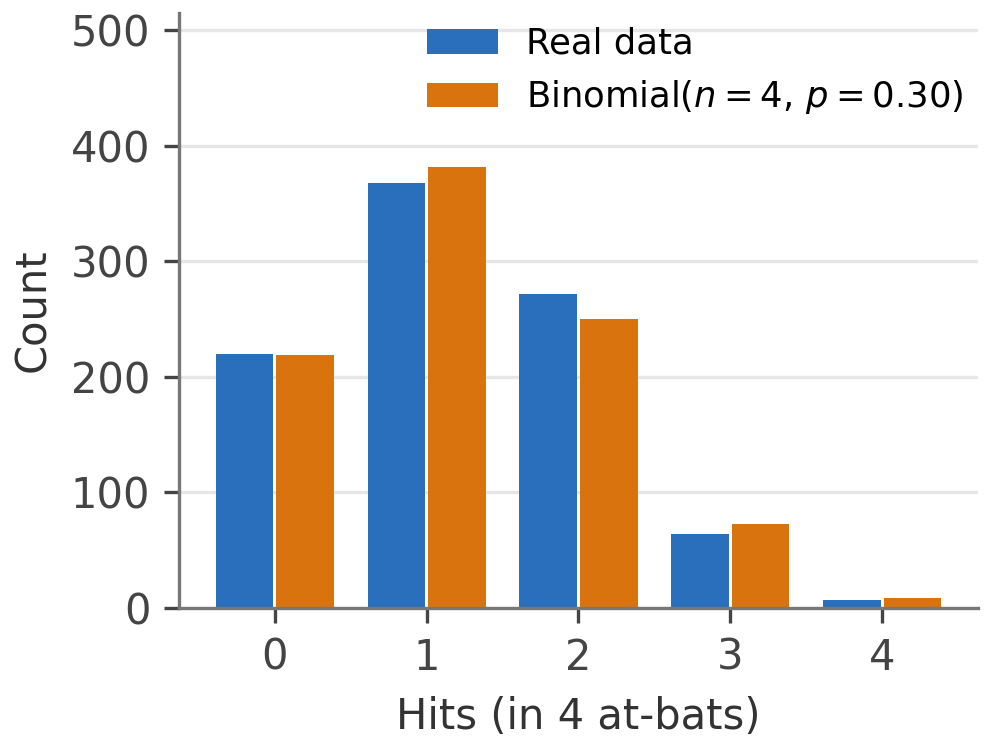
\includegraphics[width=\textwidth]{images/binomial_fit/ichiro}
}
\end{column}
\end{columns}
\end{frame}


\begin{frame}{The binomial distribution: when it doesn't fit}
\centering
\small Team wins in a season, compared to Binomial$(n, \half)$ \\[4pt]
\begin{columns}[T,onlytextwidth]
\begin{column}{0.32\textwidth}
\onslide<1->{
\centering
\textbf{NBA} {\footnotesize (2005--15)} \\[2pt]
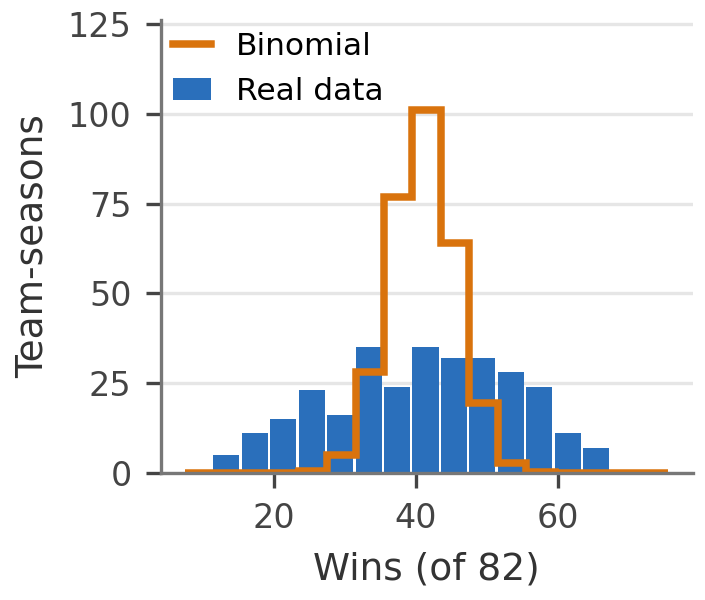
\includegraphics[width=\textwidth]{images/binomial_fit/nba_wins}
}
\end{column}
\begin{column}{0.32\textwidth}
\onslide<2->{
\centering
\textbf{NFL} {\footnotesize (2011--20)} \\[2pt]
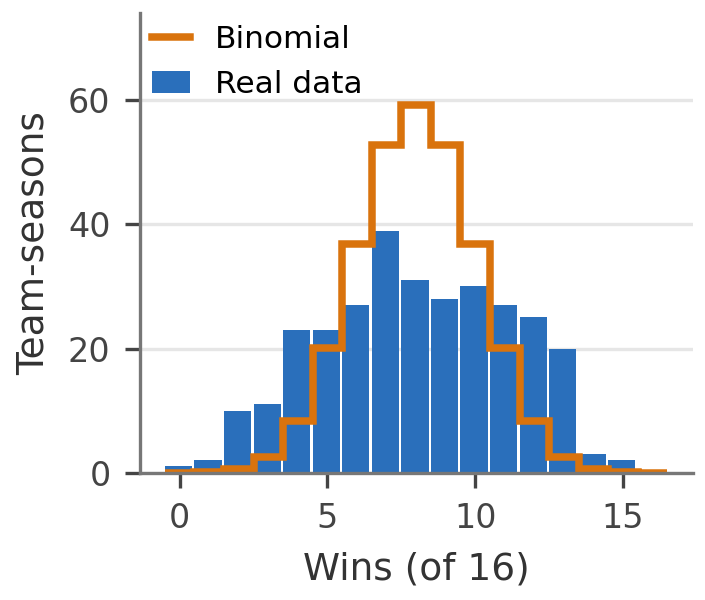
\includegraphics[width=\textwidth]{images/binomial_fit/nfl_wins}
}
\end{column}
\begin{column}{0.32\textwidth}
\onslide<3->{
\centering
\textbf{MLB} {\footnotesize (2010--19)} \\[2pt]
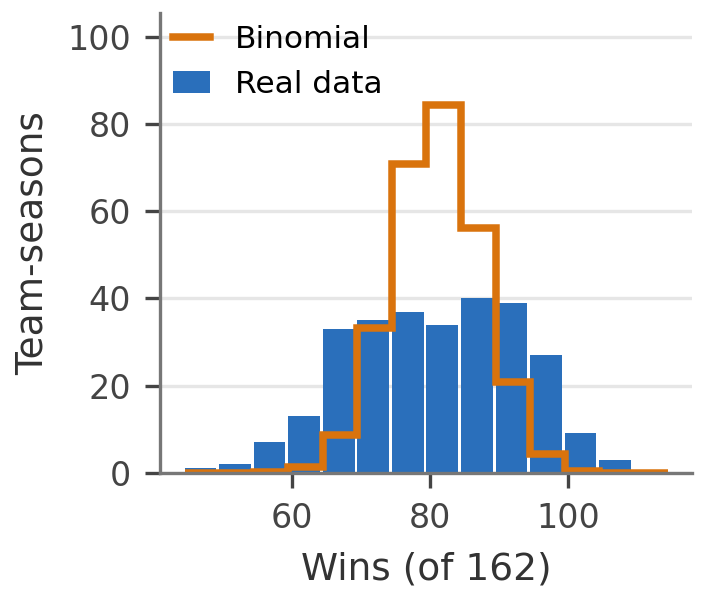
\includegraphics[width=\textwidth]{images/binomial_fit/mlb_wins}
}
\end{column}
\end{columns}
\vfill
\raggedright
\onslide<4->{\colorbox{yellow!30}{\textbf{Poll.}} Why doesn't the binomial fit?}
\vfill
\onslide<5->{\colorbox{green!30}{\textbf{Answer.}} The binomial assumes every trial has the same $p$.  But teams aren't equally good: each team has its own $p$, so win totals are far more spread out.}
\vfill
\end{frame}
